%==============================================================================
%  BINFIN -- system architecture paper
%  Elsevier (elsarticle) manuscript.  Compile with pdfLaTeX:
%      pdflatex -> pdflatex -> pdflatex      (bibliography is inline)
%==============================================================================
\documentclass[preprint,12pt,authoryear]{elsarticle}

\usepackage{amsmath}
\usepackage{amssymb}
\usepackage{booktabs}
\usepackage{graphicx}
\usepackage{multirow}
\usepackage{xcolor}
\usepackage{float}
\usepackage{algorithm}
\usepackage{algpseudocode}
\usepackage{hyperref}
\usepackage{tikz}
\usepackage{pgfplots}
\pgfplotsset{compat=1.17}
\usetikzlibrary{positioning,arrows.meta,calc,fit,backgrounds,shapes.geometric,shapes.misc}

%---- colours and node styles -------------------------------------------------
\definecolor{cIngest}{HTML}{455A64}\definecolor{cStore}{HTML}{1565C0}
\definecolor{cText}{HTML}{6A1B9A}\definecolor{cPrice}{HTML}{E65100}
\definecolor{cSig}{HTML}{00838F}\definecolor{cServe}{HTML}{2E7D32}
\definecolor{cTest}{HTML}{C62828}\definecolor{cOps}{HTML}{AD1457}
\tikzset{
  base/.style={rounded corners=2pt,draw,align=center,font=\small,minimum height=8mm,inner sep=4pt,line width=0.5pt},
  inode/.style={base,fill=cIngest!12,draw=cIngest}, snode/.style={base,fill=cStore!12,draw=cStore},
  tnode/.style={base,fill=cText!12,draw=cText},     pnode/.style={base,fill=cPrice!14,draw=cPrice},
  gnode/.style={base,fill=cSig!14,draw=cSig},       vnode/.style={base,fill=cServe!12,draw=cServe},
  rnode/.style={base,fill=cTest!12,draw=cTest},     onode/.style={base,fill=cOps!12,draw=cOps},
  group/.style={rounded corners=4pt,draw,dashed,line width=0.6pt,inner sep=6pt},
  arr/.style={-{Latex[length=2.2mm]},line width=0.7pt},
  darr/.style={-{Latex[length=2.2mm]},line width=0.7pt,dashed},
  lbl/.style={font=\scriptsize\itshape,fill=white,inner sep=1pt}}

\journal{Expert Systems with Applications}

\begin{document}

\begin{frontmatter}

\title{BINFIN: A Self-Hosted Architecture for Multi-Modal\\
       Cryptocurrency Signal Generation, and What Measuring It\\
       Revealed About Its Own Design}

\author[1]{Author One\corref{cor1}}
\ead{author1@institution.edu}
\author[1]{Author Two}
\author[2]{Author Three}

\cortext[cor1]{Corresponding author}

\affiliation[1]{organization={Department of Computer Science},
               addressline={University Name},
               city={City},
               postcode={000000},
               country={Country}}

\affiliation[2]{organization={Department of Finance},
               addressline={Institution Name},
               city={City},
               country={Country}}

\begin{abstract}
We present BINFIN, an end-to-end system that ingests cryptocurrency price, news,
social and on-chain data, scores unstructured text with a locally hosted 4-bit
quantised Mistral-7B alongside FinBERT, forecasts short-horizon direction with a
three-family model ensemble, composes explainable buy/sell/hold signals, and
simulates their execution -- all on a single commodity workstation with no
dependence on commercial model APIs. The system is $17{,}200$ lines of Python
across $169$ modules, exposing $45$ HTTP and WebSocket endpoints across eight
containerised services deployed by one command. Two architectural mechanisms are
of general interest: a \emph{hybrid split runtime} that partitions the language
model workload by function rather than by layer, pinning generation to GPU and
retrieval to CPU with capability-based fallback to CPU-only LoRA; and a
\emph{causality-by-construction} pipeline making look-ahead structurally
difficult across feature computation, scaler lifecycle, split construction and
execution semantics. The system also ships a verification harness -- $29$
regression tests, a mutation rig scoring $8/8$, and a randomised null test for
the backtester -- which is unusual for this class of system and which is the
reason the rest of this paper is possible. Turning that harness on the system
produced three concrete design defects, each quantified here. First, the
three-family ensemble does not beat its best single member on any asset, and
fitting the combination weights inverts the hand-set vector: the neural member
receives the highest fixed weight ($0.40$) but is assigned the lowest fitted
weight ($0.24$ consistently) while being the worst performer and $920\times$
slower at inference than the linear member it loses to. Second, the
rule-composed decision layer is \emph{inert}: its confidence gate is set at
$0.75$ while the maximum calibrated probability the forecasting layer ever
emits is $0.798$, so across $5{,}565$ evaluation days it fires zero signals.
Third, the forecasting layer attains $52.95\%$ directional accuracy
($p<10^{-4}$ against a coin flip) but does not separate from inverse
persistence at $52.88\%$. We report these rather than the Sharpe ratio of
$4.54$ the same system produced before the harness existed, and argue that a
platform which can locate defects in its own design is the more useful artefact.
\end{abstract}

\begin{highlights}
\item End-to-end self-hosted crypto stack: ingestion, quantised-LLM sentiment, forecasting, signals, backtesting, serving, in eight containers.
\item Hybrid split runtime partitions a 7B model workload by function, with capability-based fallback to CPU-only LoRA.
\item Verification harness (29 tests, mutation score 8/8, randomised null test) shipped as an architectural component.
\item Measured ablation: the fixed-weight ensemble beats no single member; fitted weights invert the hand-set vector.
\item Measured decision layer: the confidence gate exceeds the model's attainable output, so the rule fires zero signals.
\end{highlights}

\begin{keyword}
Trading systems \sep Self-hosted LLM \sep Quantised inference \sep QLoRA
\sep Cryptocurrency \sep System architecture \sep Ablation \sep Reproducibility
\end{keyword}

\end{frontmatter}

%==============================================================================
\section{Introduction}
\label{sec:intro}
%==============================================================================

Applied cryptocurrency research sits between two kinds of infrastructure.
Institutional platforms are capable but proprietary and unavailable for
reproduction. Public research code is generally a single notebook: a model, a
split and a printed accuracy, with no ingestion, no serving, no execution
simulation and no way to run continuously. Between them lies a gap that matters
for anyone wanting to test a market hypothesis end to end on their own hardware
and their own data, without sending that data to a third party.

BINFIN occupies that gap. It collects live price, news, social and on-chain
data; scores unstructured text with a locally hosted quantised large language
model; forecasts short-horizon direction with an ensemble; composes those outputs
into explainable signals; simulates execution with a cost- and latency-aware
backtester; and serves results over HTTP and WebSockets to a live dashboard. It
runs on one machine and requires no commercial model API.

\subsection{Design goals}

\paragraph{G1: hardware portability.} Run on a consumer GPU with 8\,GB VRAM and
degrade to CPU rather than fail. This motivates NF4 quantisation, the split
runtime of Section~\ref{ssec:runtime}, and a startup capability probe.

\paragraph{G2: data locality.} No market or user data leaves the host. This rules
out hosted LLM APIs and motivates the Ollama inference container with a local
FinBERT fallback.

\paragraph{G3: causality by construction.} Look-ahead should be structurally
difficult, not merely discouraged (Section~\ref{sec:causality}).

\paragraph{G4: verifiable claims.} Every reported number must be defensible
(Section~\ref{sec:verification}).

\subsection{Contributions}

\begin{enumerate}
    \item \textbf{A complete deployable architecture}
    (Section~\ref{sec:arch}) described in enough detail to reimplement: eight
    services, $45$ endpoints, $17{,}200$ lines of Python.
    \item \textbf{A hybrid split runtime} (Section~\ref{ssec:runtime})
    partitioning a 7B-parameter workload by function with automatic capability
    detection and two adapter configurations.
    \item \textbf{A causality-by-construction pipeline}
    (Section~\ref{sec:causality}).
    \item \textbf{A verification harness} (Section~\ref{sec:verification}):
    regression tests, mutation testing and a randomised null test, proposed as a
    baseline standard for systems of this class.
    \item \textbf{A measured self-evaluation} (Section~\ref{sec:eval}) that
    locates three quantified defects in the system's own design: an ensemble
    that does not help, a weight vector that is close to backwards, and a
    decision layer whose thresholds exceed the attainable output of the layer
    feeding it.
\end{enumerate}

\subsection{How to read the evaluation}

Section~\ref{sec:eval} reports mostly negative findings about the system's
analytical layers. We state this here rather than deferring it. The contribution
claimed is the architecture and the measurement apparatus, not a profitable
strategy. Section~\ref{ssec:caught} records that before the harness existed this
same system reported an aggregate Sharpe ratio of $4.54$ with a per-series
maximum of $23.65$, figures that were artefacts of twelve code-level faults. We
consider the ability to replace those numbers with defensible ones -- including
unflattering ones about our own design decisions -- to be the result worth
reporting.

%==============================================================================
\section{Related Work}
\label{sec:related}
%==============================================================================

\subsection{Cryptocurrency forecasting}

Most published work evaluates a model in isolation.
\citet{sezer2020financial} survey deep learning for financial time series and
note wide inconsistency in evaluation protocol. \citet{fischer2018deep} and
\citet{krauss2017deep} report on recurrent networks and tree ensembles for
equity direction with careful statistics but no deployed system.
\citet{mcnally2018predicting} apply recurrent networks to Bitcoin. Our model
families are deliberately standard; the contribution is the surrounding system
and its measurability.

\subsection{Financial text and domain models}

\citet{tetlock2007giving} established that media sentiment carries return
information, and \citet{loughran2011liability} showed general-purpose lexicons
misread financial language. FinBERT \citep{yang2020finbert}, built on BERT
\citep{devlin2019bert}, is the standard domain encoder and is our fallback path.
\citet{wu2023bloomberggpt} demonstrate the capability of large proprietary
financial models -- precisely the capability design goal G2 forgoes for locality.

\subsection{Efficient adaptation and quantised inference}

LoRA \citep{hu2022lora} adapts large models through low-rank updates; QLoRA
\citep{dettmers2023qlora} adds NF4 double-quantised backpropagation, making 7B
fine-tuning feasible on one consumer GPU. Our contribution is architectural
rather than algorithmic: how to partition such a workload in a running
multi-service system with capability-based fallback.

\subsection{Correctness in financial machine learning}

\citet{lopezdeprado2018advances} formalises purging and embargoing.
\citet{bailey2014deflated} and \citet{harvey2016cross} address selection bias in
reported performance. \citet{arnott2019backtesting} propose a backtesting
protocol for machine learning. These address statistical validity given a
correct engine; we complement them at the implementation layer, applying
mutation testing \citep{jia2011analysis} -- routine in software engineering,
rare here -- to establish that a suite detects the faults it targets.
\citet{makridakis2018statistical} document that sophisticated methods routinely
fail to beat simple benchmarks when the benchmark is actually computed, which is
the pattern Section~\ref{ssec:ablation} reproduces internally.

%==============================================================================
\section{System Architecture}
\label{sec:arch}
%==============================================================================

\begin{figure}[t]\centering
\resizebox{\textwidth}{!}{%
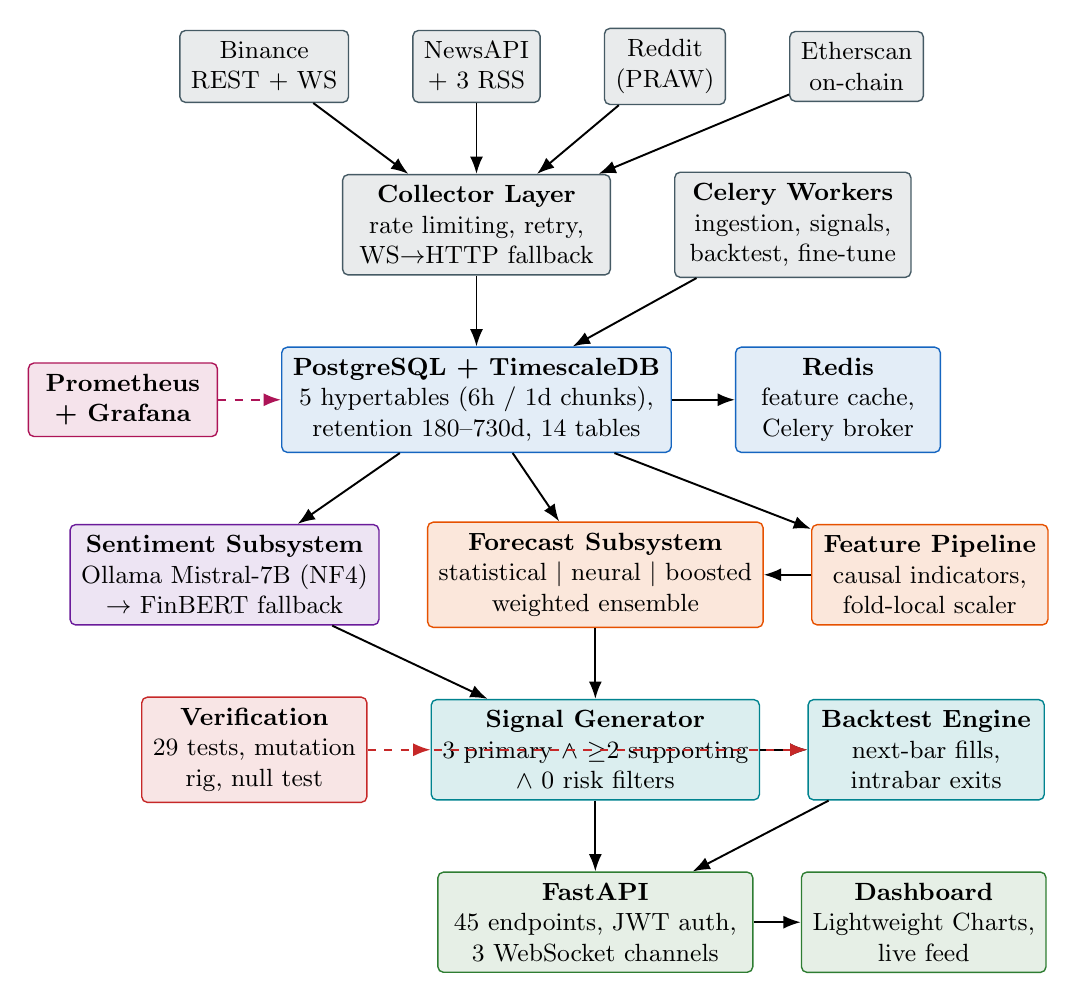
\begin{tikzpicture}[node distance=6mm and 8mm]
\node[inode] (bin)  {Binance\\ REST + WS};
\node[inode, right=of bin]  (news) {NewsAPI\\ + 3 RSS};
\node[inode, right=of news] (rdt)  {Reddit\\ (PRAW)};
\node[inode, right=of rdt]  (eth)  {Etherscan\\ on-chain};
\node[inode, below=9mm of news, minimum width=34mm] (coll)
  {\textbf{Collector Layer}\\ rate limiting, retry,\\ WS$\to$HTTP fallback};
\node[inode, right=8mm of coll, minimum width=30mm] (celery)
  {\textbf{Celery Workers}\\ ingestion, signals,\\ backtest, fine-tune};
\node[snode, below=9mm of coll, minimum width=42mm] (pg)
  {\textbf{PostgreSQL + TimescaleDB}\\ 5 hypertables (6h / 1d chunks),\\ retention 180--730d, 14 tables};
\node[snode, right=8mm of pg, minimum width=26mm] (redis)
  {\textbf{Redis}\\ feature cache,\\ Celery broker};
\node[tnode, below=9mm of pg, xshift=-32mm, minimum width=34mm] (sent)
  {\textbf{Sentiment Subsystem}\\ Ollama Mistral-7B (NF4)\\ $\to$ FinBERT fallback};
\node[pnode, right=6mm of sent, minimum width=34mm] (fc)
  {\textbf{Forecast Subsystem}\\ statistical $|$ neural $|$ boosted\\ weighted ensemble};
\node[pnode, right=6mm of fc, minimum width=30mm] (feat)
  {\textbf{Feature Pipeline}\\ causal indicators,\\ fold-local scaler};
\node[gnode, below=9mm of fc, minimum width=38mm] (sig)
  {\textbf{Signal Generator}\\ 3 primary $\wedge$ $\ge$2 supporting\\ $\wedge$ 0 risk filters};
\node[gnode, right=6mm of sig, minimum width=30mm] (bt)
  {\textbf{Backtest Engine}\\ next-bar fills,\\ intrabar exits};
\node[vnode, below=9mm of sig, minimum width=40mm] (api)
  {\textbf{FastAPI}\\ 45 endpoints, JWT auth,\\ 3 WebSocket channels};
\node[vnode, right=6mm of api, minimum width=26mm] (ui)
  {\textbf{Dashboard}\\ Lightweight Charts,\\ live feed};
\node[onode, left=8mm of pg, minimum width=24mm] (obs)
  {\textbf{Prometheus}\\ \textbf{+ Grafana}};
\node[rnode, left=8mm of sig, minimum width=24mm] (ver)
  {\textbf{Verification}\\ 29 tests, mutation\\ rig, null test};
\draw[arr] (bin)--(coll); \draw[arr] (news)--(coll); \draw[arr] (rdt)--(coll); \draw[arr] (eth)--(coll);
\draw[arr] (coll)--(pg); \draw[arr] (celery)--(pg); \draw[arr] (pg)--(redis);
\draw[arr] (pg)--(sent); \draw[arr] (pg)--(fc); \draw[arr] (pg)--(feat);
\draw[arr] (sent)--(sig); \draw[arr] (fc)--(sig); \draw[arr] (feat)--(fc);
\draw[arr] (sig)--(bt); \draw[arr] (sig)--(api); \draw[arr] (bt)--(api); \draw[arr] (api)--(ui);
\draw[darr, draw=cOps] (obs)--(pg); \draw[darr, draw=cTest] (ver)--(sig); \draw[darr, draw=cTest] (ver)--(bt);
\end{tikzpicture}}
\caption{BINFIN layered architecture. Solid arrows are data flow, dashed arrows
cross-cutting concerns. All components run as containers on one host.}
\label{fig:arch}
\end{figure}

\begin{table}[t]\centering\small
\caption{Implementation size by layer, excluding generated files and caches.}
\label{tab:components}
\begin{tabular}{@{}llr@{}}
\toprule
Layer & Principal modules & Python LOC \\
\midrule
Ingestion    & \texttt{collectors/}, \texttt{data\_ingestion/} & $\sim$1{,}900 \\
Storage      & \texttt{database.py}, schema, migrations        & $\sim$800 \\
Sentiment    & \texttt{ml/sentiment\_analyzer.py}, \texttt{api/rag.py} & $\sim$700 \\
Forecasting  & \texttt{ml/price\_predictor.py}, \texttt{ml/feature\_engineer.py}, \texttt{ml/model\_trainer.py} & $\sim$1{,}900 \\
Decision     & \texttt{signal/generator.py}, \texttt{backtest/} & $\sim$1{,}600 \\
Serving      & \texttt{api/} (45 endpoints), \texttt{main.py}   & $\sim$3{,}200 \\
Workers      & \texttt{workers/} (Celery + asyncio)             & $\sim$1{,}100 \\
Adaptation   & \texttt{llm\_trainer/}, \texttt{local\_trainer/} & $\sim$900 \\
Verification & \texttt{tests/}, \texttt{scripts/}               & $\sim$3{,}500 \\
Frontend     & dashboard (Lightweight Charts)                   & $\sim$1{,}600 \\
\midrule
\textbf{Total} & $169$ Python modules & $\mathbf{17{,}200}$ \\
\bottomrule
\end{tabular}
\end{table}

\subsection{Ingestion}

Four collectors run as supervised asyncio tasks with rate limiting, bounded
retry with exponential backoff, and graceful degradation. The price collector
consumes the Binance WebSocket stream and fails over to HTTP polling when the
socket drops, rather than stalling -- a distinction that matters because a
silently stalled feed produces stale features rather than an error. The news
collector polls NewsAPI plus three RSS feeds, deduplicating by URL and title
hash. The social collector uses PRAW with its own token-bucket limiter. The
on-chain collector crawls Etherscan with adaptive block-range sizing to stay
inside daily quotas.

\subsection{Storage}

PostgreSQL with TimescaleDB. Five high-volume tables are hypertables with chunk
intervals matched to write rate -- six hours for \texttt{price\_data}, one day
for \texttt{sentiment\_scores}, \texttt{news\_data}, \texttt{reddit\_data} and
\texttt{onchain\_transactions} -- under background retention policies ranging
from $180$ days for social data to $730$ days for prices. Fourteen tables cover
market data, derived sentiment, signals, predictions, backtest runs and trades,
users and per-user API keys. Redis serves as Celery broker and short-TTL cache
for computed feature vectors.

\subsection{Sentiment subsystem}
\label{ssec:sentiment}

\begin{figure}[t]\centering
\resizebox{0.92\textwidth}{!}{%
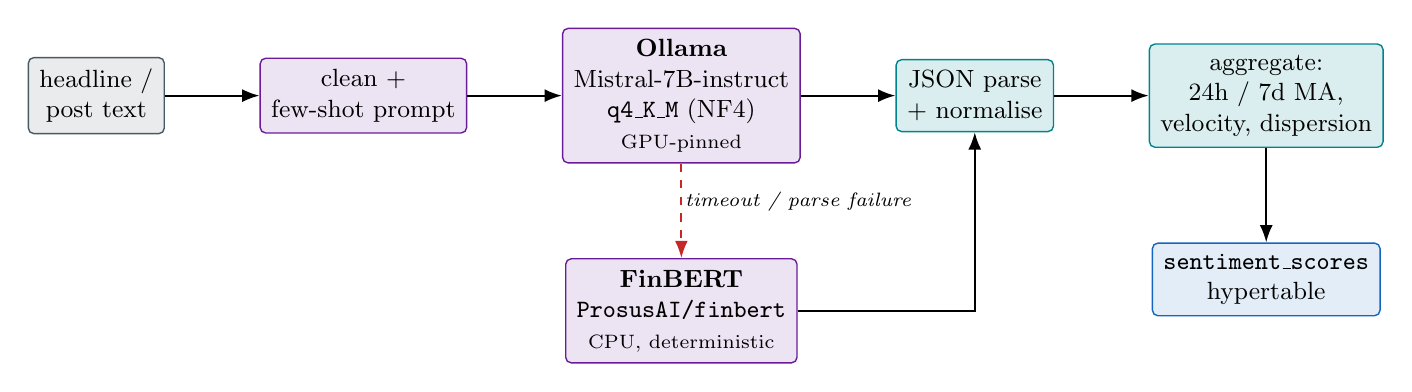
\begin{tikzpicture}[node distance=7mm and 12mm]
\node[inode] (txt) {headline /\\ post text};
\node[tnode, right=of txt] (clean) {clean +\\ few-shot prompt};
\node[tnode, right=of clean] (oll) {\textbf{Ollama}\\ Mistral-7B-instruct\\ \texttt{q4\_K\_M} (NF4)\\ \scriptsize GPU-pinned};
\node[tnode, below=12mm of oll] (fb) {\textbf{FinBERT}\\ \texttt{ProsusAI/finbert}\\ \scriptsize CPU, deterministic};
\node[gnode, right=of oll] (parse) {JSON parse\\ + normalise};
\node[gnode, right=of parse] (agg) {aggregate:\\ 24h / 7d MA,\\ velocity, dispersion};
\node[snode, below=12mm of agg] (db) {\texttt{sentiment\_scores}\\ hypertable};
\draw[arr] (txt)--(clean); \draw[arr] (clean)--(oll); \draw[arr] (oll)--(parse);
\draw[arr] (parse)--(agg); \draw[arr] (agg)--(db);
\draw[darr, draw=cTest] (oll.south) -- node[lbl,right,pos=0.4]{timeout / parse failure} (fb.north);
\draw[arr] (fb.east) -| (parse.south);
\end{tikzpicture}}
\caption{Dual-path sentiment scoring. The quantised generative model is primary;
FinBERT is a deterministic fallback on timeout or malformed output.}
\label{fig:sentiment}
\end{figure}

The primary path sends a few-shot prompt to a Mistral-7B-instruct model quantised
to \texttt{q4\_K\_M}, served by Ollama in its own container, constrained to emit
JSON carrying a label, a confidence and a short reasoning string. The reasoning
is retained and surfaced in the dashboard, which is what makes signals
inspectable rather than opaque. On timeout or unparseable output the request
falls through to FinBERT on CPU, which is deterministic and fast but produces no
rationale. Scores are aggregated into 24-hour and 7-day moving averages, a
velocity term and a dispersion term.

\subsection{Forecasting subsystem}
\label{ssec:forecast}

Three model families are trained per asset and combined:
\begin{itemize}
\item a \textbf{statistical} member (Prophet in the deployed configuration) for
trend and seasonality decomposition with exogenous regressors;
\item a \textbf{neural} member, a stacked LSTM classifier over windows of the
feature matrix with early stopping;
\item a \textbf{boosted} member (XGBoost) over the flattened window, retaining
feature importances.
\end{itemize}
Component probabilities are combined by a fixed weighting,
\begin{equation}
P_{\text{ens}}(c) = 0.30\,P_{\text{stat}}(c) + 0.40\,P_{\text{neural}}(c) + 0.30\,P_{\text{boost}}(c).
\label{eq:ensemble}
\end{equation}
Section~\ref{ssec:ablation} tests this weighting empirically, with results that
do not support it.

\subsection{Decision layer}
\label{ssec:signal}

The decision layer is rule-composed rather than learned, so every signal carries
a human-readable justification. A BUY requires all three primary conditions, at
least two of five supporting conditions, and zero of four risk filters:
\begin{equation}
\textsc{buy} \iff |\mathcal{P}| = 3 \;\wedge\; |\mathcal{S}| \ge 2 \;\wedge\; |\mathcal{R}| = 0 ,
\label{eq:signal}
\end{equation}
with sets as in Table~\ref{tab:signal}. SELL mirrors it; anything else is HOLD.
A cooldown suppresses repeats on the same symbol.

\begin{table}[t]\centering\small
\caption{BUY conditions. The conjunction over $\mathcal{P}$ is the binding
constraint, as Section~\ref{ssec:decision} shows.}
\label{tab:signal}
\begin{tabular}{@{}lll@{}}
\toprule
Set & Condition & Threshold \\
\midrule
\multirow{3}{*}{Primary $\mathcal{P}$}
 & 24h aggregate sentiment      & $> 0.70$ \\
 & Ensemble direction label     & $=$ UP \\
 & Ensemble confidence          & $> 0.75$ \\
\midrule
\multirow{5}{*}{Supporting $\mathcal{S}$}
 & Net exchange flow            & $< 0$ \\
 & RSI(14)                      & $< 40$ \\
 & 24h volume ratio             & $> 1.0$ \\
 & Sentiment velocity           & $> 0$ \\
 & News sentiment delta         & $> 0$ \\
\midrule
\multirow{4}{*}{Risk $\mathcal{R}$}
 & 1-period drawdown            & $< -10\%$ \\
 & ATR ratio                    & $> 2.0$ \\
 & Negative exchange news flag  & set \\
 & Regulatory FUD flag          & set \\
\bottomrule
\end{tabular}
\end{table}

\subsection{Execution simulation}
\label{ssec:backtest}

The backtester is bar-driven rather than signal-driven: it iterates the union of
bar timestamps, resolving exits for open positions against \emph{that position's
own} asset bar, then opening positions scheduled for that bar, then closing
positions whose bar-counted holding period has expired. Three semantics matter:
a signal from the close of bar $i$ is scheduled for bar $i+1$ and filled at its
open, so no fill can reference information at or after its own execution bar;
stops and targets resolve against each bar's high and low, with ties going
pessimistically to the stop; and equity carries shorts as a liability,
$V_t = \text{cash}_t + \sum_{\text{long}} q_j p_t^{(j)} - \sum_{\text{short}} q_j p_t^{(j)}$,
with each leg charged fees on its own notional.

\subsection{Hybrid split runtime}
\label{ssec:runtime}

\begin{figure}[t]\centering
\resizebox{0.95\textwidth}{!}{%
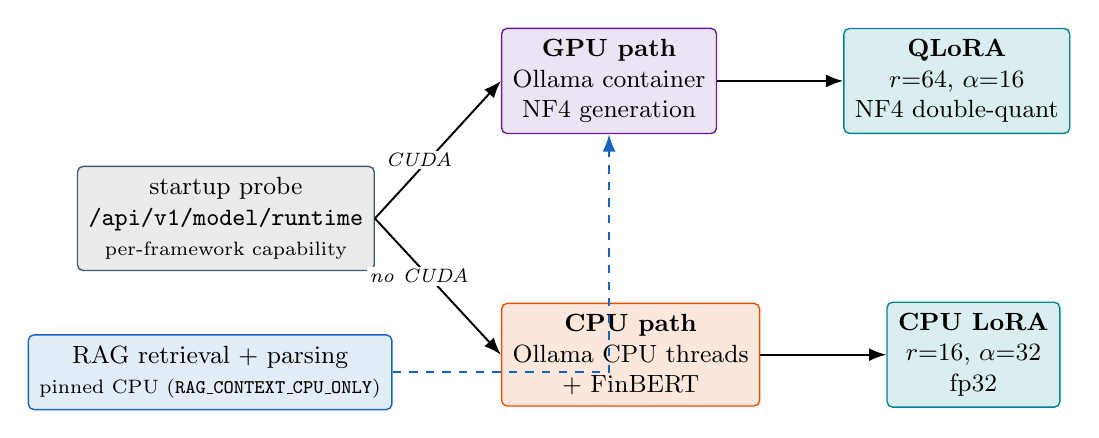
\begin{tikzpicture}[node distance=6mm and 10mm]
\node[inode] (probe) {startup probe\\ \texttt{/api/v1/model/runtime}\\ \scriptsize per-framework capability};
\node[tnode, above right=4mm and 16mm of probe] (gpu) {\textbf{GPU path}\\ Ollama container\\ NF4 generation};
\node[pnode, below right=4mm and 16mm of probe] (cpu) {\textbf{CPU path}\\ Ollama CPU threads\\ + FinBERT};
\node[gnode, right=16mm of gpu] (qlora) {\textbf{QLoRA}\\ $r{=}64$, $\alpha{=}16$\\ NF4 double-quant};
\node[gnode, right=16mm of cpu] (lora) {\textbf{CPU LoRA}\\ $r{=}16$, $\alpha{=}32$\\ fp32};
\node[snode, below=8mm of probe, xshift=-2mm] (rag) {RAG retrieval + parsing\\ \scriptsize pinned CPU (\texttt{RAG\_CONTEXT\_CPU\_ONLY})};
\draw[arr] (probe.east) -- node[lbl,above,pos=0.35]{CUDA} (gpu.west);
\draw[arr] (probe.east) -- node[lbl,below,pos=0.35]{no CUDA} (cpu.west);
\draw[arr] (gpu)--(qlora); \draw[arr] (cpu)--(lora);
\draw[darr, draw=cStore] (rag.east) -| (gpu.south);
\end{tikzpicture}}
\caption{Capability-based runtime selection. Generation is GPU-pinned when CUDA
is present; retrieval and parsing are always CPU-resident to preserve VRAM.}
\label{fig:runtime}
\end{figure}

The partition is by \emph{function}, not by layer. Token generation, the
VRAM-hungry and latency-critical operation, runs in the GPU-enabled Ollama
container. Retrieval-augmented context assembly -- embedding lookup, database
routing, prompt construction -- is pinned to CPU by configuration, because it is
memory-bandwidth rather than compute bound and would otherwise consume VRAM the
model needs.

At startup the backend probes accelerator availability and reports a runtime
plan. If CUDA is absent or VRAM insufficient, inference falls back to CPU threads
and fine-tuning switches from QLoRA to CPU LoRA. The two adapter configurations
differ deliberately (Table~\ref{tab:qlora}): NF4 quantisation frees enough memory
to support a substantially higher adapter rank than the CPU path can hold in
fp32. Trained adapters are packaged into an Ollama Modelfile and registered as a
local tag, so serving consumes a fine-tuned model through the same interface as
the base model.

\begin{table}[t]\centering\small
\caption{Adapter configurations for the two training paths.}
\label{tab:qlora}
\begin{tabular}{@{}lll@{}}
\toprule
& GPU (QLoRA) & CPU (LoRA) \\
\midrule
Base weights      & NF4, double-quantised & fp32 \\
Adapter rank $r$  & $64$ & $16$ \\
$\alpha$          & $16$ & $32$ \\
Dropout           & $0.05$ & $0.05$ \\
Target modules    & \multicolumn{2}{l}{\texttt{q,k,v,o\_proj}, \texttt{gate,up,down\_proj}} \\
\bottomrule
\end{tabular}
\end{table}

\subsection{Serving, workers and observability}

FastAPI exposes $45$ endpoints spanning market data, sentiment, predictions,
signals, backtests, model operations, JWT authentication and per-user API key
management, plus three WebSocket channels pushing ticks and signal
notifications. Long-running work is offloaded to Celery: ingestion supervision,
scheduled signal generation, backtest execution, and fine-tuning jobs with a
24-hour limit and cancellation. Prometheus counters instrument ingestion restarts
and per-task errors, scraped into Grafana dashboards provisioned as code. The
stack is eight Compose services brought up by one command, with a GPU overlay for
CUDA hosts.

%==============================================================================
\section{Causality by Construction}
\label{sec:causality}
%==============================================================================

Four mechanisms implement design goal G3.

\paragraph{Causal features.} Every feature is a function of bars indexed $\le t$.
Rolling statistics use trailing windows; window normalisation is per-lookback
rather than global, so no statistic is informed by data after the observation it
describes.

\paragraph{Scaler lifecycle.} The scaler is fitted on training rows only,
persisted with the model artefacts, and applied at inference through
\texttt{transform}. The separation is enforced by the API surface: the serving
path has no method that fits. Absent a fitted scaler the system warns and returns
unscaled features rather than silently producing a degenerate vector.

\paragraph{Embargoed splits.} Because samples are overlapping windows with
next-bar labels, splits discard a gap
\begin{equation}
\mathcal{T}_{\text{train}} = [0, k), \quad
\mathcal{T}_{\text{test}} = [k + e, n), \quad e \ge L_{\text{seq}} + h,
\label{eq:embargo}
\end{equation}
following \citet{lopezdeprado2018advances}.

\paragraph{Execution semantics.} Bar lookup is constrained to
$\{i : t_i \le t_{\text{signal}}\}$ by binary search, making it structurally
impossible for a fill to resolve against a future bar.

%==============================================================================
\section{Verification Harness}
\label{sec:verification}
%==============================================================================

\subsection{Regression suite}

Twenty-nine tests use fixtures with analytically known answers rather than
database data, so they run without infrastructure. They cover no-look-ahead
fills, per-asset position pricing, short accounting, intrabar exit resolution,
holding-period semantics, Sharpe annualisation against its closed form, bootstrap
non-degeneracy, scaler behaviour and split disjointness. The strongest is a
closed-loop invariant: with all positions flat at the end,
\begin{equation}
V_T - V_0 = \sum_{i=1}^{N} \mathrm{PnL}_i
\label{eq:reconcile}
\end{equation}
must hold exactly. Any fault creating or destroying cash violates it, and it
cannot be satisfied by accident.

\subsection{Mutation testing}
\label{ssec:mutation}

A test count measures effort, not coverage. A pytest plugin reintroduces one
known fault before collection, selected by environment variable, and a driver
runs the suite once per fault.

\begin{table}[t]\centering\small
\caption{Mutation results against a green baseline of $29$ tests.}
\label{tab:mutation}
\begin{tabular}{@{}llr@{}}
\toprule
Reintroduced fault & Detected by & Red \\
\midrule
Look-ahead bar lookup          & \texttt{price\_lookup\_never\_selects\_future\_bar} & 1 \\
Inverted short mark-to-market  & \texttt{short\_equity\_falls\_when\_price\_rises}   & 1 \\
Evenly split round-trip fee    & \texttt{equity\_curve\_reconciles\_with\_trade\_pnl}& 1 \\
Per-trade Sharpe annualisation & \texttt{annualisation\_matches\_closed\_form} (+1)  & 2 \\
Permutation-invariant bootstrap& \texttt{bootstrap\_is\_not\_degenerate}             & 1 \\
Scaler refit at transform      & \texttt{single\_row\_transform\_not\_all\_zeros} (+1)& 2 \\
Split without embargo          & \texttt{gap\_between\_folds} (+1)                   & 2 \\
Close-only exit checks         & \texttt{stop\_fills\_at\_stop\_level} (+1)          & 2 \\
\midrule
\multicolumn{2}{@{}l}{\textbf{Mutation score}} & $\mathbf{8/8}$ \\
\bottomrule
\end{tabular}
\end{table}

Five further faults are covered by dedicated tests but are not separately
expressible as isolated mutations without rewriting the simulation loop; we
exclude them from the score rather than counting them for free.

\subsection{Randomised null test}

Random signals on a driftless geometric random walk contain no structure by
construction, so a correct engine charging positive costs must lose at a rate set
by turnover and cost alone. The assertion must be distributional: a $75$-day
fixture has $\mathrm{SE}(S) \approx 2.2$, and measured over $60$ seeds,
$13.3\%$ produce a positive Sharpe. Over those seeds $\bar{S} = -3.534$,
$\mathrm{se} = 0.470$, $t = -7.51$, with cash conservation holding to
$1.2\times10^{-11}$ on runs ending flat.

This exercises the \emph{engine} with exogenous signals. It is blind to feature,
split and imputation leakage upstream, and is one necessary check among several.

%==============================================================================
\section{Evaluation}
\label{sec:eval}
%==============================================================================

All measurements below were taken on the host in Table~\ref{tab:host}.

\begin{table}[t]\centering\small
\caption{Measurement host.}
\label{tab:host}
\begin{tabular}{@{}ll@{}}
\toprule
CPU & Intel, 10 physical / 16 logical cores \\
RAM & $16.9$\,GB \\
GPU & NVIDIA GeForce RTX 4060 Laptop \\
OS / Python & Windows 11 / CPython 3.12 \\
\bottomrule
\end{tabular}
\end{table}

\subsection{Component latency and throughput}
\label{ssec:latency}

\begin{table}[t]\centering\small
\caption{Measured latency and throughput. Inference percentiles over $200$
repetitions ($60$ for the LSTM), single-sample batches, warm process.}
\label{tab:latency}
\begin{tabular}{@{}lrrrr@{}}
\toprule
Operation & p50 (ms) & p95 (ms) & p99 (ms) & Notes \\
\midrule
Scaler transform      & $0.052$  & $0.060$  & $0.073$  & 34 features \\
Logistic inference    & $0.054$  & $0.066$  & $0.134$  & \\
Boosted inference     & $2.333$  & $4.060$  & $4.669$  & 200 trees, depth 3 \\
\textbf{LSTM inference}& $\mathbf{49.685}$ & $\mathbf{77.673}$ & $\mathbf{118.739}$ & CPU, 30-step window \\
\midrule
\multicolumn{5}{@{}l}{\emph{Throughput}} \\
Feature construction  & \multicolumn{3}{l}{$3{,}150$ bars in $17.8$\,ms $= 5.7\,\mu$s/bar} & \\
Backtest engine       & \multicolumn{3}{l}{$18{,}000$ bars, $4{,}474$ trades in $0.06$\,s $= 293{,}479$ bars/s} & \\
Process RSS           & \multicolumn{3}{l}{$1{,}448$\,MB with all three model families loaded} & \\
\bottomrule
\end{tabular}
\end{table}

Per-fold training costs $0.01$\,s for the linear member, $0.14$--$0.39$\,s for
the boosted member and $1.80$--$2.45$\,s for the LSTM.

The ratio worth noting is that the LSTM costs $920\times$ the linear member at
inference ($49.685$ vs $0.054$\,ms) and roughly $200\times$ at training.
Section~\ref{ssec:ablation} shows what that buys.

\subsection{Runtime heterogeneity: a deployment finding}
\label{ssec:heterogeneity}

The capability probe of Section~\ref{ssec:runtime} was designed on the assumption
that accelerator availability is a property of the host. It is not: it is a
property of the \emph{host and framework pair}. On the measurement host, PyTorch
reports CUDA available and enumerates the RTX 4060, while TensorFlow reports zero
GPUs -- native Windows GPU support was dropped in TensorFlow $\ge 2.11$, and is
available only through WSL2 or a DirectML plugin.

The consequence is that on this host the QLoRA fine-tuning path (PyTorch) runs on
GPU while the LSTM forecasting path (Keras) silently runs on CPU, on the same
machine, at the same time. A probe returning a single boolean would have reported
``GPU available'' and been wrong for half the stack. This is the reason the LSTM
latency in Table~\ref{tab:latency} is a CPU figure, and it is a concrete argument
for capability detection being per-framework rather than per-host -- a
generalisable lesson for any multi-framework deployment.

\subsection{Ablation: does the ensemble help?}
\label{ssec:ablation}

Equation~\eqref{eq:ensemble} combines three families with hand-set weights.
Nothing established that the combination beats its best member, or that the fixed
weights beat fitted ones. We test both under the walk-forward protocol, training
all arms on the same inner-training block so the comparison is fair, and fitting
weights on a held-out validation slice inside the training fold by grid search
over the simplex.

Two substitutions are forced by the environment and are stated because they
matter: Prophet and XGBoost are optional dependencies not installed here, so the
statistical slot is filled by regularised logistic regression and the boosted
slot by histogram gradient boosting. The LSTM is the real Keras model.
Conclusions about \emph{ensembling} transfer; conclusions about Prophet
specifically do not.

\begin{table}[t]\centering\small
\caption{Ablation. ``vs best single'' is a paired comparison on identical days
against the best-performing individual member, which is the linear model on all
three assets.}
\label{tab:ablation}
\begin{tabular}{@{}llrrcr@{}}
\toprule
Asset & Arm & $n$ & Accuracy & 95\% CI & vs best single \\
\midrule
\multirow{7}{*}{BTC}
 & Statistical (linear)  & $2{,}084$ & $\mathbf{52.98\%}$ & $[50.8, 55.1]$ & --- \\
 & Boosted               & $2{,}084$ & $51.44\%$ & $[49.3, 53.6]$ & --- \\
 & \textbf{Neural (LSTM)}& $2{,}084$ & $50.29\%$ & $[48.1, 52.4]$ & --- \\
 & Ensemble, equal       & $2{,}084$ & $52.93\%$ & $[50.8, 55.1]$ & $-0.05$pp ($p=0.96$) \\
 & Ensemble, deployed    & $2{,}084$ & $52.74\%$ & $[50.6, 54.9]$ & $-0.24$pp ($p=0.81$) \\
 & Ensemble, fitted      & $2{,}084$ & $53.45\%$ & $[51.3, 55.6]$ & $+0.48$pp ($p=0.53$) \\
 & \textit{Inverse persistence} & $2{,}084$ & \textit{53.02\%} & --- & --- \\
\midrule
\multirow{7}{*}{ETH}
 & Statistical (linear)  & $2{,}084$ & $\mathbf{50.91\%}$ & $[48.8, 53.1]$ & --- \\
 & Boosted               & $2{,}084$ & $50.29\%$ & $[48.1, 52.4]$ & --- \\
 & Neural (LSTM)         & $2{,}084$ & $50.62\%$ & $[48.5, 52.8]$ & --- \\
 & Ensemble, equal       & $2{,}084$ & $50.62\%$ & $[48.5, 52.8]$ & $-0.29$pp ($p=0.76$) \\
 & Ensemble, deployed    & $2{,}084$ & $50.77\%$ & $[48.6, 52.9]$ & $-0.14$pp ($p=0.88$) \\
 & Ensemble, fitted      & $2{,}084$ & $51.34\%$ & $[49.2, 53.5]$ & $+0.43$pp ($p=0.68$) \\
 & \textit{Inverse persistence} & $2{,}084$ & \textit{52.54\%} & --- & --- \\
\midrule
\multirow{7}{*}{DOGE}
 & Statistical (linear)  & $1{,}397$ & $\mathbf{52.90\%}$ & $[50.3, 55.5]$ & --- \\
 & Boosted               & $1{,}397$ & $50.89\%$ & $[48.3, 53.5]$ & --- \\
 & \textbf{Neural (LSTM)}& $1{,}397$ & $48.89\%$ & $[46.3, 51.5]$ & --- \\
 & Ensemble, equal       & $1{,}397$ & $51.83\%$ & $[49.2, 54.4]$ & $-1.07$pp ($p=0.38$) \\
 & Ensemble, deployed    & $1{,}397$ & $51.54\%$ & $[48.9, 54.2]$ & $-1.36$pp ($p=0.27$) \\
 & Ensemble, fitted      & $1{,}397$ & $51.11\%$ & $[48.5, 53.7]$ & $-1.79$pp ($p=0.09$) \\
 & \textit{Inverse persistence} & $1{,}397$ & \textit{53.11\%} & --- & --- \\
\bottomrule
\end{tabular}
\end{table}

Three results follow.

\paragraph{The ensemble beats no single member.} On every asset, the best
individual model is the linear one, and no ensemble variant improves on it
significantly. On DOGE all three ensemble variants are \emph{worse}, the fitted
variant by $1.79$ percentage points ($p = 0.09$). Averaging a good model with two
worse ones degrades it, which is what averaging does when the members are not
independently informative.

\paragraph{The deployed weight vector is close to backwards.} The fitted weights
in Table~\ref{tab:weights} put the least weight on the neural member on every
asset, at a strikingly stable $0.24$, while the deployed configuration gives it
the \emph{most} at $0.40$. The statistical member, which the deployed vector ties
for least at $0.30$, is fitted at $0.46$--$0.59$.

\begin{table}[t]\centering\small
\caption{Fitted versus deployed ensemble weights. Fitted values are means over
walk-forward folds, obtained on validation slices inside the training fold.}
\label{tab:weights}
\begin{tabular}{@{}lccc@{}}
\toprule
& Statistical & Neural & Boosted \\
\midrule
Deployed (Eq.~\ref{eq:ensemble}) & $0.30$ & $\mathbf{0.40}$ & $0.30$ \\
Fitted, BTC  & $0.59$ & $\mathbf{0.24}$ & $0.16$ \\
Fitted, ETH  & $0.46$ & $\mathbf{0.24}$ & $0.30$ \\
Fitted, DOGE & $0.55$ & $\mathbf{0.24}$ & $0.21$ \\
\bottomrule
\end{tabular}
\end{table}

\paragraph{Compute is allocated inversely to value.} Combining
Table~\ref{tab:latency} with Table~\ref{tab:ablation}: the neural member is the
worst performer on all three assets, is the only member to fall below $50\%$ on
any asset ($48.89\%$ on DOGE), receives the highest deployed weight, and costs
$920\times$ the inference latency of the member that beats it. This is the
clearest single finding of the evaluation, and it is a finding about our
architecture rather than about the data.

\subsection{Decision layer: the rule is inert}
\label{ssec:decision}

The decision layer had never been measured. We evaluate it on the same
walk-forward predictions, using real calibrated \texttt{predict\_proba} output
rather than a placeholder.

One condition cannot be evaluated. The BUY rule requires a 24-hour aggregate
sentiment above $0.70$, and the only historical sentiment series available is
synthetic -- generated from same-day returns, correlating $0.916$ with the
contemporaneous return and $-0.018$ with the next day's -- and is excluded from
all results. We therefore evaluate the rule with the sentiment primary
\emph{removed}, which is the most generous possible treatment: it can only
increase the firing rate.

\begin{table}[t]\centering\small
\caption{Decision-layer funnel, sentiment gate removed. Columns are cumulative
survivors. Zero signals fire on any asset.}
\label{tab:decision}
\begin{tabular}{@{}lrrrrr@{}}
\toprule
Asset & Candidates & Pass $\mathcal{P}$ & Pass $\mathcal{S}$ & Pass $\mathcal{R}$ & Fired \\
\midrule
BTC   & $2{,}084$ & $2$  & $2$ & $0$ & $\mathbf{0}$ \\
ETH   & $2{,}084$ & $17$ & $6$ & $0$ & $\mathbf{0}$ \\
DOGE  & $1{,}397$ & $2$  & $2$ & $0$ & $\mathbf{0}$ \\
\bottomrule
\end{tabular}
\end{table}

\begin{table}[t]\centering\small
\caption{Why the funnel closes: the confidence gate exceeds what the forecasting
layer can produce.}
\label{tab:gate}
\begin{tabular}{@{}lrrr@{}}
\toprule
Asset & Gate & Max $P(\uparrow)$ ever observed & Days above gate \\
\midrule
BTC   & $0.75$ & $0.798$ & $0.096\%$ \\
ETH   & $0.75$ & $0.922$ & $0.816\%$ \\
DOGE  & $0.75$ & $0.850$ & $0.143\%$ \\
\bottomrule
\end{tabular}
\end{table}

The system as configured emits no signals at all. The cause is a distribution
mismatch: the confidence gate was set at $0.75$ without reference to the output
distribution of the layer feeding it, and a calibrated model on a signal this
weak almost never exceeds it -- BTC's maximum over $2{,}084$ days is $0.798$, and
fewer than one day in a thousand clears the threshold. The handful that do are
then eliminated by the risk filters, because high model confidence coincides with
high realised volatility, which is exactly what the ATR filter is designed to
reject.

This is a genuine architectural defect, and it is one that no amount of testing
the \emph{components} would have surfaced: each layer is individually correct.
It appears only when the layers are measured against each other.

\subsection{Predictive evaluation}
\label{ssec:predictive}

Evaluated on Binance spot daily bars with expanding-window walk-forward
validation, a $5$-day embargo, a $1{,}000$-day initial training block and
$250$-day test folds, with the scaler fitted inside each fold. Out-of-sample
coverage is $5{,}562$ predictions from 2020-07-17 to 2026-03-30.

\begin{table}[t]\centering\small
\caption{Out-of-sample directional accuracy with Wilson intervals. Inverse
persistence is a zero-parameter rule betting against the previous day's
direction.}
\label{tab:acc}
\begin{tabular}{@{}llrrcr@{}}
\toprule
Asset & Predictor & $n$ & Accuracy & 95\% CI & $p$ vs $.5$ \\
\midrule
\multirow{3}{*}{BTC}
 & Forecasting layer            & $2{,}083$ & $52.71\%$ & $[50.6, 54.8]$ & $0.013$ \\
 & \textbf{Inverse persistence} & $2{,}083$ & $\mathbf{53.00\%}$ & $[50.9, 55.1]$ & $0.006$ \\
 & Majority class               & $2{,}083$ & $50.55\%$ & $[48.4, 52.7]$ & $0.614$ \\
\midrule
\multirow{3}{*}{ETH}
 & Forecasting layer            & $2{,}083$ & $53.10\%$ & $[50.9, 55.2]$ & $0.005$ \\
 & Inverse persistence          & $2{,}083$ & $52.57\%$ & $[50.4, 54.7]$ & $0.019$ \\
 & Majority class               & $2{,}083$ & $49.59\%$ & $[47.4, 51.8]$ & $0.710$ \\
\midrule
\multirow{3}{*}{DOGE}
 & Forecasting layer            & $1{,}396$ & $53.08\%$ & $[50.5, 55.7]$ & $0.021$ \\
 & \textbf{Inverse persistence} & $1{,}396$ & $\mathbf{53.15\%}$ & $[50.5, 55.7]$ & $0.019$ \\
 & Majority class               & $1{,}396$ & $51.72\%$ & $[49.1, 54.3]$ & $0.199$ \\
\midrule
\multirow{2}{*}{\textbf{Pooled}}
 & \textbf{Forecasting layer}   & $5{,}562$ & $\mathbf{52.95\%}$ & $[51.6, 54.3]$ & $<10^{-4}$ \\
 & \textbf{Inverse persistence} & $5{,}562$ & $\mathbf{52.88\%}$ & $[51.6, 54.2]$ & $<10^{-4}$ \\
\bottomrule
\end{tabular}
\end{table}

Against a coin flip the forecasting layer works, with Pesaran--Timmermann
$p$-values of $0.015$, $0.008$ and $0.016$ confirming genuine directional
dependence. Against inverse persistence it does not: paired comparisons on
identical days give $-0.29$, $+0.53$ and $-0.07$ percentage points with
$|t| \le 0.45$, and the system loses on two of three assets. What the pipeline
has learned is the documented one-day reversal effect.

Two diagnostics sharpen this. The return-weighted hit rate is \emph{below} the
unweighted accuracy on every asset ($51.68$, $51.57$, $52.33$ against $52.71$,
$53.10$, $53.08$), so the signal concentrates in small moves. And gating on model
confidence degrades net Sharpe monotonically from $+0.113$ to $-0.309$ -- the
ensemble confidence of Section~\ref{ssec:forecast} is mildly anti-informative,
which is the same property that makes the decision layer inert.

\subsection{Economic evaluation}

\begin{table}[t]\centering\small
\caption{Book statistics, equal-weight daily long/short, costs of 4\,bps taker
plus 5\,bps slippage per side.}
\label{tab:book}
\begin{tabular}{@{}lrrrrr@{}}
\toprule
Weighting & $\mu$ (\%/yr) & $\sigma$ (\%/yr) & SR gross & SR net & Turnover \\
\midrule
Equal        & $+6.61$ & $58.38$ & $+0.544$ & $+0.113$ & $0.765$ \\
Inverse-vol  & $+4.25$ & $55.14$ & $+0.527$ & $+0.077$ & $0.755$ \\
\bottomrule
\end{tabular}
\end{table}

The gross Sharpe of $0.544$ carries a stationary-bootstrap
\citep{politis1994stationary} $95\%$ interval of $[-0.172, +1.285]$, containing
zero. Breakeven transaction cost is $11.4$\,bps per side with an interval of
$[0, 26.9]$, containing the assumed $9$. Against a passive equal-weight basket
the correlation is $+0.224$, beta $+0.215$, and the appraisal ratio $-0.076$.

A decomposition isolating one change at a time attributes the frictionless-to-executed
gap to transaction costs ($-0.431$ Sharpe) and holding-period effects
($-0.144$); the one-bar entry lag costs $+0.001$, because cryptocurrency trades
continuously and close-to-open dispersion is $1.6\%$ of intraday dispersion.

\subsection{What the harness caught}
\label{ssec:caught}

Before the harness existed, this system reported an aggregate annualised Sharpe
of $4.54$ with a per-series maximum of $23.65$. Those figures were artefacts of
twelve code-level faults, including exits priced from the wrong asset's bar; a
bar lookup that could resolve into the future; Sharpe computed by annualising
per-trade returns with a fixed $\sqrt{252}$; shorts marked to market with the
wrong sign; a Monte Carlo routine that shuffled a P\&L vector and summed it,
which is permutation-invariant and therefore constant; and a feature scaler
fitted on a single row at inference, which returns identically zero, so every
served prediction ran on a zero vector.

Several survived long review because they \emph{compensate}: the inverted short
accounting corrupted the equity curve, but Sharpe was computed from the trade
record and never touched it. This is the argument for testing the instrument
directly rather than inspecting outputs for plausibility.

%==============================================================================
\section{Discussion}
\label{sec:discussion}
%==============================================================================

\subsection{Three defects, and what they have in common}

The evaluation located three defects in our own design: an ensemble that helps
nothing, a weight vector approximately inverted relative to the fitted optimum,
and a decision layer whose gate exceeds the attainable output of the layer
feeding it.

They share a cause. Each is an \emph{interface} property, invisible from inside
any single component. The LSTM is correctly implemented; it is simply not
informative on this data, which only a paired ablation reveals. The weights are
applied correctly; they are just wrong, which only fitting reveals. The
confidence gate is correctly evaluated; it is just unreachable, which only
measuring the joint distribution of two layers reveals. Unit tests over
components would pass in every case. This suggests that systems of this shape
need a category of test we did not have -- assertions on the \emph{joint}
behaviour of adjacent layers, such as that a downstream threshold lies inside the
observed range of its upstream input.

\subsection{What the negative predictive result implicates}

The result in Section~\ref{ssec:predictive} concerns a specific configuration:
thirty-four single-asset technical features, a daily horizon, retail taker costs.
The ingestion, storage, serving and verification layers are agnostic to what is
predicted. What is implicated is the feature set -- which omits every
crypto-specific microstructure signal, including perpetual funding, open
interest, basis, liquidation cascades, order-book imbalance and cross-asset
lead--lag -- and the training objective, which is log-loss on direction when the
binding constraint turns out to be transaction cost.

\subsection{The value of a system that can find its own faults}

Most systems in this class cannot produce the findings in
Sections~\ref{ssec:ablation} and \ref{ssec:decision}, because they lack the
apparatus to look. The same codebase that now reports a zero firing rate reported
a Sharpe ratio of $4.54$ eighteen months earlier and was believed. The difference
is not the models; it is that the measurement layer is now calibrated, shipped
and re-runnable by a reader.

\subsection{Explainability as an architectural property}

The generative sentiment path returns a stored reasoning string, and the decision
layer is rule-composed, so every signal carries the conditions that fired. This
costs predictive flexibility -- a learned decision layer would plausibly fire
more often and better -- and is a deliberate trade for a system meant to be
audited by its operator. Section~\ref{ssec:decision} shows the trade was priced
wrongly, not that it was wrong in principle.

%==============================================================================
\section{Limitations}
\label{sec:limitations}
%==============================================================================

\paragraph{Ablation substitutions.} Prophet and XGBoost were unavailable in the
measurement environment and were substituted by logistic regression and
histogram gradient boosting. Conclusions about ensembling transfer; conclusions
about Prophet specifically do not, and re-running with the deployed members
remains outstanding.

\paragraph{Sentiment path unvalidated.} The live sentiment subsystem is not
evaluated anywhere in this paper. The only historical series available is
synthetic and excluded, so no claim here concerns sentiment-driven prediction,
and the sentiment primary in Equation~\eqref{eq:signal} remains untested.

\paragraph{Benchmarks are offline-path only.} Table~\ref{tab:latency} measures
feature construction, model inference and backtest throughput. It does not
measure end-to-end request latency through FastAPI, WebSocket delivery,
ingestion throughput against live APIs, or GPU memory under concurrent load,
all of which require a running deployment with live credentials.

\paragraph{LLM inference not benchmarked.} Ollama generation latency and VRAM
occupancy are unmeasured, because the container was not running on the
measurement host. Given Section~\ref{ssec:heterogeneity}, these should be
reported per framework and per accelerator rather than as single figures.

\paragraph{Cost model.} A flat $4$\,bps taker plus $5$\,bps slippage is likely
conservative for BTC and ETH at daily horizon, where passive execution is
feasible. A defensible passive assumption would move the point estimate above
breakeven, though not outside its confidence interval.

\paragraph{Instrument idealisation.} We model Binance spot but evaluate a
long/short book, which requires margin. Funding, borrow availability and
liquidation are not modelled.

\paragraph{Mutation coverage.} Eight of thirteen expressible faults are covered
by the mutation rig; five are covered only by direct tests.

\paragraph{Single-node.} No horizontal scaling, multi-tenant isolation, capacity
analysis, or live/paper-trading validation.

%==============================================================================
\section{Conclusion}
\label{sec:conclusion}
%==============================================================================

We described BINFIN, a self-hosted system that ingests multi-modal
cryptocurrency data, analyses text with a locally hosted 4-bit quantised
Mistral-7B alongside FinBERT, forecasts direction with a model ensemble,
composes explainable signals, simulates execution and serves the result --
$17{,}200$ lines of Python, $45$ endpoints, eight containers, one command to
deploy, on a $16$\,GB workstation.

Three elements transfer beyond this application: a hybrid split runtime that
partitions a large-model workload by function and degrades by capability, which
Section~\ref{ssec:heterogeneity} shows must be detected per framework rather than
per host; a causality-by-construction pipeline spanning features, scaler
lifecycle, splits and execution; and a verification harness -- $29$ tests, a
mutation score of $8/8$, a randomised null test -- shipped as an architectural
component.

Turning that harness on the system produced three quantified defects in our own
design. The three-family ensemble beats no single member, and the deployed
weights are close to inverted: the neural member carries the highest fixed weight
and the lowest fitted weight, is the worst performer on all three assets, and
costs $920\times$ the inference latency of the linear model that beats it. The
rule-composed decision layer is inert, because its confidence gate of $0.75$
exceeds the $0.798$ maximum the forecasting layer ever attains. And the
forecasting layer, while distinguishable from a coin flip at $p<10^{-4}$, is not
distinguishable from inverse persistence.

We report these instead of the Sharpe ratio of $4.54$ the same system produced
before the harness existed. The architecture is what we offer; the defects it
found in itself are the evidence that the architecture works.

%==============================================================================
\section*{Reproducibility}
%==============================================================================

Source: \url{https://github.com/Ratnachand04/FINBIN}, commit
\texttt{83a31ac}. Evaluation data are daily Binance klines committed to the
repository; SHA-256 prefixes are \texttt{aca018e6c7c299b1} (BTCUSDT, $3{,}151$
rows), \texttt{20a0bef67dd349b2} (ETHUSDT, $3{,}151$ rows) and
\texttt{5eefe6147b3820b3} (DOGEUSDT, $2{,}464$ rows).

Every table in Section~\ref{sec:eval} regenerates from a single command:
\texttt{evaluate\_walkforward.py} (Tables~\ref{tab:acc}, \ref{tab:book}),
\texttt{ablation\_and\_benchmark.py} (Tables~\ref{tab:latency},
\ref{tab:ablation}, \ref{tab:weights}), \texttt{decision\_layer\_study.py}
(Tables~\ref{tab:decision}, \ref{tab:gate}), \texttt{mutation\_matrix.py}
(Table~\ref{tab:mutation}) and \texttt{null\_test\_backtest.py}. Numerical
output is serialised to \texttt{docs/*.json}.

%==============================================================================
\appendix
%==============================================================================

\section{Selected API surface}
\label{app:api}

\begin{table}[H]\centering\small
\caption{Representative endpoints of the $45$ exposed; prefix \texttt{/api/v1}
omitted.}
\begin{tabular}{@{}lll@{}}
\toprule
Group & Path & Purpose \\
\midrule
Market      & \texttt{/coins/\{symbol\}/price-history}        & OHLCV series \\
Market      & \texttt{/coins/\{symbol\}/technical-indicators} & derived indicators \\
Sentiment   & \texttt{/sentiment/\{symbol\}/sentiment-history}& scored text series \\
Sentiment   & \texttt{/sentiment/aggregate}                   & windowed aggregates \\
Prediction  & \texttt{/predictions/latest}                    & ensemble output \\
Signals     & \texttt{/signals/active}                        & open signals \\
Signals     & \texttt{/signals/\{id\}/execute}                & mark executed \\
Backtest    & \texttt{/backtest/run}                          & launch run \\
Model ops   & \texttt{/model/runtime}                         & capability probe \\
Model ops   & \texttt{/model/finetune}                        & launch adapter job \\
LLM         & \texttt{/llm/generate}                          & RAG-backed generation \\
Stream      & \texttt{/ws/live-data}                          & tick push \\
Stream      & \texttt{/ws/notifications}                      & signal push \\
\bottomrule
\end{tabular}
\end{table}

\section{Storage schema}
\label{app:schema}

Fourteen tables; five are TimescaleDB hypertables: \texttt{price\_data}
($6$-hour chunks, $730$-day retention), \texttt{sentiment\_scores} and
\texttt{onchain\_transactions} ($1$-day chunks, $365$-day retention), and
\texttt{news\_data} and \texttt{reddit\_data} ($1$-day chunks, $180$-day
retention). Remaining relations cover \texttt{trading\_signals},
\texttt{predictions}, \texttt{backtest\_runs}, \texttt{backtest\_trades},
\texttt{model\_metadata}, \texttt{users} and \texttt{user\_api\_keys}.

%==============================================================================
\begin{thebibliography}{99}
%==============================================================================

\bibitem[Arnott et~al.(2019)]{arnott2019backtesting}
Arnott, R., Harvey, C.~R., Markowitz, H., 2019.
A backtesting protocol in the era of machine learning.
Journal of Financial Data Science 1 (1), 64--74.

\bibitem[Bailey and L\'opez de Prado(2014)]{bailey2014deflated}
Bailey, D.~H., L\'opez de Prado, M., 2014.
The deflated Sharpe ratio.
Journal of Portfolio Management 40 (5), 94--107.

\bibitem[Dettmers et~al.(2023)]{dettmers2023qlora}
Dettmers, T., Pagnoni, A., Holtzman, A., Zettlemoyer, L., 2023.
QLoRA: efficient finetuning of quantized LLMs.
In: Advances in Neural Information Processing Systems 36.

\bibitem[Devlin et~al.(2019)]{devlin2019bert}
Devlin, J., Chang, M.-W., Lee, K., Toutanova, K., 2019.
BERT: pre-training of deep bidirectional transformers for language understanding.
In: Proceedings of NAACL-HLT, pp. 4171--4186.

\bibitem[Fischer and Krauss(2018)]{fischer2018deep}
Fischer, T., Krauss, C., 2018.
Deep learning with long short-term memory networks for financial market
predictions.
European Journal of Operational Research 270 (2), 654--669.

\bibitem[Harvey et~al.(2016)]{harvey2016cross}
Harvey, C.~R., Liu, Y., Zhu, H., 2016.
$\dots$ and the cross-section of expected returns.
Review of Financial Studies 29 (1), 5--68.

\bibitem[Hu et~al.(2022)]{hu2022lora}
Hu, E.~J., Shen, Y., Wallis, P., Allen-Zhu, Z., Li, Y., Wang, S., Wang, L.,
Chen, W., 2022.
LoRA: low-rank adaptation of large language models.
In: International Conference on Learning Representations.

\bibitem[Jia and Harman(2011)]{jia2011analysis}
Jia, Y., Harman, M., 2011.
An analysis and survey of the development of mutation testing.
IEEE Transactions on Software Engineering 37 (5), 649--678.

\bibitem[Krauss et~al.(2017)]{krauss2017deep}
Krauss, C., Do, X.~A., Huck, N., 2017.
Deep neural networks, gradient-boosted trees, random forests: statistical
arbitrage on the S\&P 500.
European Journal of Operational Research 259 (2), 689--702.

\bibitem[L\'opez de Prado(2018)]{lopezdeprado2018advances}
L\'opez de Prado, M., 2018.
Advances in Financial Machine Learning.
Wiley, Hoboken, NJ.

\bibitem[Loughran and McDonald(2011)]{loughran2011liability}
Loughran, T., McDonald, B., 2011.
When is a liability not a liability? Textual analysis, dictionaries, and 10-Ks.
Journal of Finance 66 (1), 35--65.

\bibitem[Makridakis et~al.(2018)]{makridakis2018statistical}
Makridakis, S., Spiliotis, E., Assimakopoulos, V., 2018.
Statistical and machine learning forecasting methods: concerns and ways forward.
PLoS ONE 13 (3), e0194889.

\bibitem[McNally et~al.(2018)]{mcnally2018predicting}
McNally, S., Roche, J., Caton, S., 2018.
Predicting the price of Bitcoin using machine learning.
In: 26th Euromicro International Conference on Parallel, Distributed and
Network-based Processing, pp. 339--343.

\bibitem[Politis and Romano(1994)]{politis1994stationary}
Politis, D.~N., Romano, J.~P., 1994.
The stationary bootstrap.
Journal of the American Statistical Association 89 (428), 1303--1313.

\bibitem[Sezer et~al.(2020)]{sezer2020financial}
Sezer, O.~B., Gudelek, M.~U., Ozbayoglu, A.~M., 2020.
Financial time series forecasting with deep learning: a systematic literature
review, 2005--2019.
Applied Soft Computing 90, 106181.

\bibitem[Tetlock(2007)]{tetlock2007giving}
Tetlock, P.~C., 2007.
Giving content to investor sentiment: the role of media in the stock market.
Journal of Finance 62 (3), 1139--1168.

\bibitem[Wu et~al.(2023)]{wu2023bloomberggpt}
Wu, S., Irsoy, O., Lu, S., Dabravolski, V., Dredze, M., Gehrmann, S., Kambadur,
P., Rosenberg, D., Mann, G., 2023.
BloombergGPT: a large language model for finance.
arXiv preprint arXiv:2303.17564.

\bibitem[Yang et~al.(2020)]{yang2020finbert}
Yang, Y., Uy, M. C.~S., Huang, A., 2020.
FinBERT: a pretrained language model for financial communications.
arXiv preprint arXiv:2006.08097.

\end{thebibliography}

\end{document}
